\section*{MHVAE's}
\begin{frame}{Markovian Hierarchical Variational Autoencoder (MHVAE)}
    \begin{figure}
        \centering
        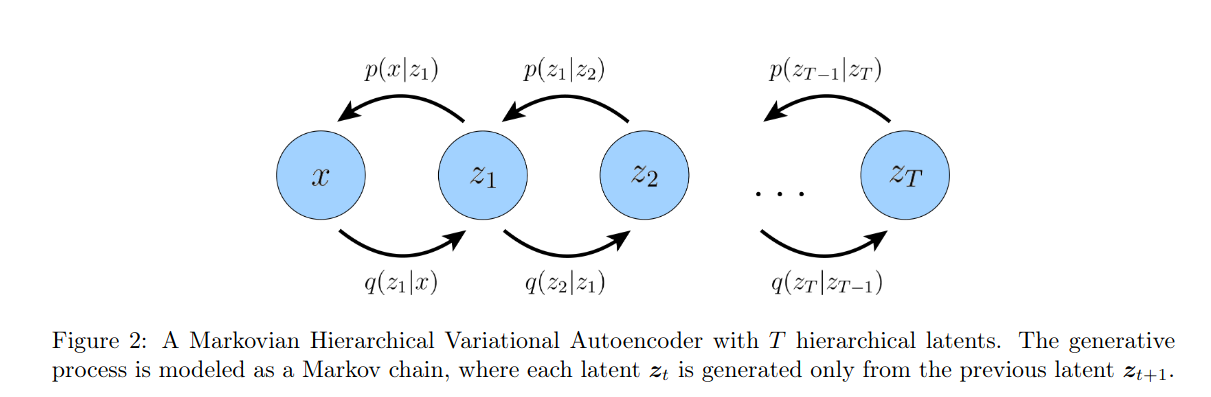
\includegraphics[width=1\textwidth]{Images/hvae1.png}
        \caption{Markovian Hierarchical Variational Autoencoder}
    \end{figure}

    In MHVAE, we have a hierarchical structure of latent variables. 
\end{frame}

\begin{frame}{Markovian Hierarchical Variational Autoencoder (MHVAE)}
    Now we have a hierarchical structure of latent variables.
    $z_1, z_2, \ldots, z_T$ are the latent variables at each time step. We can denote all these using $z_{1:T}$.
\end{frame}

\begin{frame}{Joint and Posterior}
    The Joint Distribution can be written as:  
    \begin{align*}
        p(x, z_{1:T}) &= p(z_T)p(x|z_1) \prod_{t=2}^{T} p(z_{t-1}|z_t)
    \end{align*}

    The posterior distribution can be written as:
    \begin{align*}
        p(z_{1:T}|x) &= \frac{p(x, z_{1:T})}{p(x)} \\
        &= \frac{p(x)p(z_1|x) \prod_{t=2}^{T} p(z_{t}|z_{t-1})}{p(x)} \\
        &= p(z_1|x) \prod_{t=2}^{T} p(z_{t}|z_{t-1}) \\
    \end{align*}
\end{frame}

\begin{frame}{Extending ELBO}
    \begin{align*}
        \log(p(x)) &= \log \left( \int p(x, z_{1:T}) dz_{1:T} \right) \\
        &= \log \left( \int p(x, z_{1:T}) \frac{q(z_{1:T}|x)}{q(z_{1:T}|x)} dz_{1:T} \right) \\
        &= \log \left( \mathbb{E}_{q(z_{1:T}|x)} \left[ \frac{p(x, z_{1:T})}{q(z_{1:T}|x)} \right] \right) \\
        &\geq \mathbb{E}_{q(z_{1:T}|x)} \left[ \log \left( \frac{p(x, z_{1:T})}{q(z_{1:T}|x)} \right) \right] && \text{(Jensen's Inequality)} \\
    \end{align*}
\end{frame}

\begin{frame}{Extending ELBO}
    \begin{align*}
        \log(p(x)) &\geq \mathbb{E}_{q(z_{1:T}|x)} \left[ \log \left( \frac{p(x, z_{1:T})}{q(z_{1:T}|x)} \right) \right] \\
        &= \mathbb{E}_{q(z_{1:T}|x)} \left[ \log \left( \frac{p(z_T)p(x|z_1) \prod_{t=2}^{T} p(z_{t-1}|z_t)}{q(z_{1:T}|x)} \right) \right] \\
        &= \mathbb{E}_{q(z_{1:T}|x)} \left[ \log \left( \frac{p(z_T)p(x|z_1) \prod_{t=2}^{T} p(z_{t-1}|z_t)}{q(z_1|x) \prod_{t=2}^{T} q(z_t|z_{t-1})} \right) \right] \\
    \end{align*}

    We will see how this expression can be broken down into terms that we have seen in VAE.
\end{frame}